\refstepcounter{section}
\section*{Lecture 15: Curvatures}
\addcontentsline{toc}{section}{Lecture 15: Curvatures}
We try to develop a physical interpretation of the Ricci tensor. Note that this contains a \textit{double derivative} of the metric, that is $\partial_\alpha\partial_\beta g_{\mu\nu}$. 
\begin{figure}[H]
    \centering 
    

\tikzset{every picture/.style={line width=0.75pt}} %set default line width to 0.75pt        

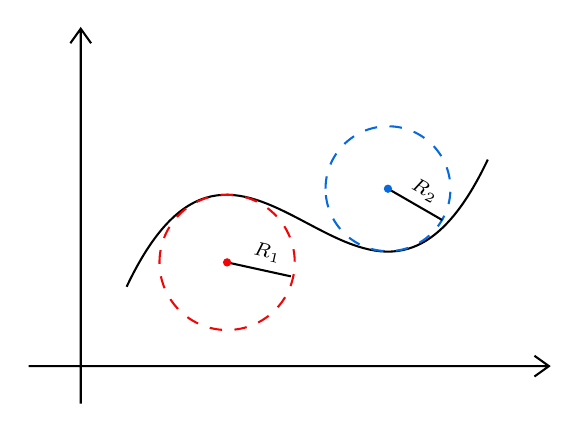
\begin{tikzpicture}[x=0.75pt,y=0.75pt,yscale=-1,xscale=1]
%uncomment if require: \path (0,300); %set diagram left start at 0, and has height of 300

%Shape: Axis 2D [id:dp38924385912108406] 
\draw  (141,204.57) -- (391.65,204.57)(166.06,42) -- (166.06,222.63) (384.65,199.57) -- (391.65,204.57) -- (384.65,209.57) (161.06,49) -- (166.06,42) -- (171.06,49)  ;
%Shape: Polynomial [id:dp3727956568654499] 
\draw   (188.17,166.33) .. controls (246.17,43.8) and (304.18,227.6) .. (362.18,105.07) ;
%Shape: Circle [id:dp9266249134268983] 
\draw  [color={rgb, 255:red, 240; green, 6; blue, 6 }  ,draw opacity=1 ][dash pattern={on 4.5pt off 4.5pt}] (204,154.58) .. controls (204,136.59) and (218.59,122) .. (236.58,122) .. controls (254.58,122) and (269.17,136.59) .. (269.17,154.58) .. controls (269.17,172.58) and (254.58,187.17) .. (236.58,187.17) .. controls (218.59,187.17) and (204,172.58) .. (204,154.58) -- cycle ;
%Straight Lines [id:da042806453509152464] 
\draw    (236.58,154.58) -- (267.31,161.32) ;
%Shape: Circle [id:dp7368572411766657] 
\draw  [color={rgb, 255:red, 240; green, 6; blue, 6 }  ,draw opacity=1 ][fill={rgb, 255:red, 240; green, 6; blue, 6 }  ,fill opacity=1 ] (235.12,154.58) .. controls (235.12,155.39) and (235.78,156.05) .. (236.58,156.05) .. controls (237.39,156.05) and (238.05,155.39) .. (238.05,154.58) .. controls (238.05,153.78) and (237.39,153.12) .. (236.58,153.12) .. controls (235.78,153.12) and (235.12,153.78) .. (235.12,154.58) -- cycle ;
%Shape: Circle [id:dp0112281968788156] 
\draw  [color={rgb, 255:red, 6; green, 106; blue, 221 }  ,draw opacity=1 ][dash pattern={on 4.5pt off 4.5pt}] (284,119.09) .. controls (284,102.47) and (297.47,89) .. (314.09,89) .. controls (330.71,89) and (344.18,102.47) .. (344.18,119.09) .. controls (344.18,135.71) and (330.71,149.18) .. (314.09,149.18) .. controls (297.47,149.18) and (284,135.71) .. (284,119.09) -- cycle ;
%Straight Lines [id:da49138136587987] 
\draw    (314.09,119.09) -- (340.18,134.15) ;
%Shape: Circle [id:dp015878606441429133] 
\draw  [color={rgb, 255:red, 6; green, 106; blue, 221 }  ,draw opacity=1 ][fill={rgb, 255:red, 6; green, 106; blue, 221 }  ,fill opacity=1 ] (312.63,119.09) .. controls (312.63,119.9) and (313.28,120.55) .. (314.09,120.55) .. controls (314.9,120.55) and (315.55,119.9) .. (315.55,119.09) .. controls (315.55,118.28) and (314.9,117.63) .. (314.09,117.63) .. controls (313.28,117.63) and (312.63,118.28) .. (312.63,119.09) -- cycle ;

% Text Node
\draw (249.29,142.89) node [anchor=north west][inner sep=0.75pt]  [font=\scriptsize,rotate=-12.6]  {$R_{1}$};
% Text Node
\draw (327.36,111.43) node [anchor=north west][inner sep=0.75pt]  [font=\scriptsize,rotate=-28.64]  {$R_{2}$};


\end{tikzpicture}

\end{figure}
\noindent
Suppose we have some arbitrary smooth curve. Then, at each point of the curve, we can associate a circle whose first and second derivatives match with that of the curve. And there is always a radius associated with such a circle. Thus, to each point on the curve, we can associate a radius $r$, referred to as the \textit{radius of curvature} of the curve at that point. \\[0.2cm]
Now, for simplicity, let us assume that at a point $P$ on the curve, we have drawn the circle and we shifted our origin to $P$. Thus, the equation of the circle becomes: 
$$x^2+y^2=r^2$$
From the equation of the circle, we obtain,
$$y\dv{y}{x} + x = 0 \implies y \dv[2]{y}{x} + \qty(\dv{y}{x})+1 = 0 \implies y = \frac{1+\qty(\dv{y}{x})^2}{-\dv[2]{y}{x}}$$
Also, from above, we have $$\dv{y}{x} = -\frac{x}{y}$$
Then we obtain an expression for the radius of the circle:
\begin{align*}
    r = \Big|\sqrt{x^2+y^2}\big| &=\Bigg|y\sqrt{1+\qty(\frac{x}{y})^2}\Bigg|\\
    &=\Bigg| \frac{1+\qty(\dv{y}{x})^2}{-\dv[2]{y}{x}} \times \sqrt{1+\qty(\frac{x}{y})^2}\Bigg|\\
    &=\Biggr|\frac{\qty[1+\qty(\dv{y}{x})^2]^{\sfrac{3}{2}}}{\dv[2]{y}{x}} \Biggr|
\end{align*}
By choosing an appropriate coordinate system, we can always set the first derivative to zero \footnote{Note that since first derivative roughly gives us the maxima or the minima, with proper rotation and shifting of the coordinates, we can indeed make those points to be zero.} and we have a result that,
$$r = \Bigg|\dv[2]{y}{x}\Bigg|^{-1}$$
Thus, the second derivative represents the curvature of the curve, since it is intrinsically related to the radius of curvature. And since the Ricci/Riemann tensor contains double derivative of the metric, it somehow represents the curvature of the space. Hence, it is sometimes also called \textit{Riemann curvature tensor}!\\[0.2cm]
Now, for the sake of getting our hands dirty, let us calculate the Ricci scalar of $\mathbb{S}^2$ (sphere), of radius $r_0$. 
\begin{figure}[H]
    \centering 
    

\tikzset{every picture/.style={line width=0.75pt}} %set default line width to 0.75pt        

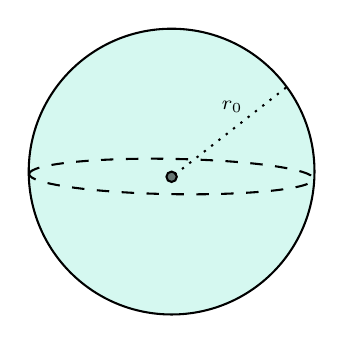
\begin{tikzpicture}[x=0.75pt,y=0.75pt,yscale=-1,xscale=1]
%uncomment if require: \path (0,232); %set diagram left start at 0, and has height of 232

%Shape: Circle [id:dp8457214999849747] 
\draw  [fill={rgb, 255:red, 80; green, 227; blue, 194 }  ,fill opacity=0.24 ] (220.57,135.84) .. controls (220.57,97.82) and (251.39,67) .. (289.41,67) .. controls (327.43,67) and (358.25,97.82) .. (358.25,135.84) .. controls (358.25,173.86) and (327.43,204.68) .. (289.41,204.68) .. controls (251.39,204.68) and (220.57,173.86) .. (220.57,135.84) -- cycle ;
%Shape: Ellipse [id:dp187786419702904] 
\draw  [dash pattern={on 4.5pt off 4.5pt}] (220.8,137.01) .. controls (220.88,132.32) and (251.61,129.05) .. (289.44,129.71) .. controls (327.27,130.37) and (357.87,134.71) .. (357.79,139.4) .. controls (357.71,144.09) and (326.98,147.36) .. (289.15,146.7) .. controls (251.32,146.04) and (220.72,141.7) .. (220.8,137.01) -- cycle ;
%Shape: Circle [id:dp9969910330717426] 
\draw  [fill={rgb, 255:red, 0; green, 0; blue, 0 }  ,fill opacity=0.52 ] (286.92,138.34) .. controls (286.92,139.72) and (288.03,140.83) .. (289.41,140.83) .. controls (290.79,140.83) and (291.91,139.72) .. (291.91,138.34) .. controls (291.91,136.96) and (290.79,135.84) .. (289.41,135.84) .. controls (288.03,135.84) and (286.92,136.96) .. (286.92,138.34) -- cycle ;
%Straight Lines [id:da9228343591459383] 
\draw  [dash pattern={on 0.84pt off 2.51pt}]  (290.91,137.34) -- (344.97,95.03) ;

% Text Node
\draw (312,100.4) node [anchor=north west][inner sep=0.75pt]  [font=\scriptsize]  {$r_{0}$};


\end{tikzpicture}

\end{figure}
\noindent
For this, we first need to calculate the Riemann tensor, then contract it to get Ricci tensor and then again contract it to get Ricci scalar. Thus, this seems a very involved task and we have to do that carefully!\\[0.2cm]
As calculate before, the metric for the sphere is written as:
$$ds^2 = r_0^2\dd\theta^2 + r_0^2\sin^2\theta\dd\phi^2 $$
From there we get the metric tensor and inverse metric tensor as:
$$g_{\mu\nu} = \mathrm{diag}(r_0^2, r_0^2\sin^2\theta)\qquad g^{\mu\nu} = \mathrm{diag}(\sfrac{1}{r_0^2}, \sfrac{1}{r_0^2\sin^2\theta})$$
Also, we had earlier found that only two of the Christoffel symbols are non-zero, namely,
$$\chris{\theta}{\phi}{\phi}=-\sin\theta \cos\theta \qquad \chris{\phi}{\theta}{\phi} = \cot\theta$$
\underline{Calculating the Riemann Tensor}
$$\rie{\rho}{\sigma}{\mu}{\nu} = \partial_\mu \chris{\rho}{\nu}{\sigma} + \chris{\rho}{\mu}{\lambda}\chris{\lambda}{\nu}{\sigma} -\partial_\nu \chris{\rho}{\mu}{\sigma} - \chris{\rho}{\nu}{\lambda}\chris{\lambda}{\mu}{\sigma}  $$
Let us take $\rho =\theta, \sigma = \phi, \mu=\theta, \nu = \phi$ first. Then we have:
\begin{align*}
    \rie{\theta}{\phi}{\theta}{\phi} &= \partial_\theta \chris{\theta}{\phi}{\phi} + \chris{\theta}{\theta}{\lambda}\chris{\lambda}{\phi}{\phi} -\partial_\phi \chris{\theta}{\theta}{\phi} - \chris{\theta}{\phi}{\lambda}\chris{\lambda}{\theta}{\phi} \\
    &=-\partial_\theta \qty(\frac{1}{2}\sin 2\theta) + \sin\theta\cos\theta \times \cos\theta\\
    &=-\frac{1}{2}\cos 2\theta +\cancel{ \sin\theta}\cos\theta \times \frac{\cos\theta}{\cancel{ \sin\theta}}\\
    &=\sin^2\theta-\cos^2\theta +\cos^2\theta\\
    &=\sin^2\theta
\end{align*}
In fact, this is the only non-zero Riemann tensor component. Other components will be zero owing to the anti-symmetric and other nice properties of the Riemann tensor. \\[0.2cm]
\underline{Calculating the Ricci Tensor}
$$R_{\mu}{\nu} = \rie{\lambda}{\mu}{\lambda}{\nu}$$
We calculate the components one by one.
\begin{align*}
    R_{\theta\theta} & = \rie{\lambda}{\theta}{\lambda}{\theta}
\end{align*}
Note that we only found out one component of the Riemann tensor. We have to transform all quantitites to that form only. Here, the only non-zero index will be $\lambda=\phi$, thus we get,
\begin{align*}
    R_{\theta\theta} &= \rie{\phi}{\theta}{\phi}{\theta}\\
    &=g^{\phi\alpha}R_{\alpha \theta \phi \theta}\\
    &=g^{\phi\alpha} (-1)(-1)R_{\theta \alpha \theta \phi }\\
    &=g^{\phi\phi} R_{\theta \phi \theta \phi } \qquad \text{($\because g$ diagonal, so $\alpha = \phi$)}\\
    &=\frac{1}{r_0^2\sin^2\theta} g_{\theta\sigma}\rie{\sigma}{\phi}{\theta}{\phi }\\
    &=\frac{1}{r_0^2\sin^2\theta} r_0^2\rie{\theta}{\phi}{\theta}{\phi }\qquad \text{($\because g$ diagonal, so $\sigma = \theta$)}\\
    &=1
\end{align*}
$R_{\theta\phi} = 0$ due to the anti-symmetric property and $R_{\phi\phi} = \rie{\lambda}{\phi}{\lambda}{\phi} =\rie{\theta}{\phi}{\theta}{\phi} =\sin^2\theta$. Now, we have obtained all the components of the Ricci tensor and hence, let us move on to the Ricci scalar. 
\begin{align*}
    R = \tensor{R}{^\mu _\mu} = g^{\mu\nu}R_{\mu\nu} = \frac{1}{r_0^2}\times 1 + \frac{1}{r_0^2\sin^2\theta}\times \sin^2\theta = \frac{2}{r_0^2}
\end{align*}
Thus we obtain that the Ricci scalar for the sphere is $\frac{2}{r_0^2}$. Thus, the Ricci scalar indeed refers to the usual curvature and its inverse represents the radius of curvature!
$$R^{-1}\sim r_0^2$$